\graphicspath{{lectures/03_eloadas_abrak/}}

\section{A kezdetiérték-probléma létezése és egyértelműsége}

\subsection{A kezdetiérték-problémával ekvivalens integrálegyenlet}

Tekintsük az
\[
 \begin{cases}
   x'=f\circ(\operatorname{id},x),\\
   x(\tau)=\xi
 \end{cases}
 \qquad\text{kezdetiérték-problémát (k.é.p.).}
\]

\noindent\textbf{Tétel.} Ha $\varphi$ megoldása a k.é.p.-nak, akkor $\exists$
$I\subseteq\mathbb R$ nyílt intervallum és egy deriválható
$\varphi:I\to\mathbb R^n$ függvény úgy, hogy
\[
 \varphi'(t)=f\bigl(t,\varphi(t)\bigr),\qquad
 \varphi(\tau)=\xi.
\]
Integrálva:
\[
 \boxed{\displaystyle
 \varphi(t)=\xi+\int_\tau^t f\bigl(s,\varphi(s)\bigr)\,ds},
 \qquad t\in I.
\]

Ez motiválja a következő feladatot: adott $n\in\mathbb N$,
$f:D\to\mathbb R^n$, ahol $D\subseteq\mathbb R\times\mathbb R^n$
tartomány és $f$ folytonos. Keressünk $I\subseteq\mathbb R$
nyílt intervallumot és folytonos $\varphi:I\to\mathbb R^n$
függvényt, amelyre
\[
 \varphi(t)=\xi+\int_\tau^t f\bigl(s,\varphi(s)\bigr)\,ds
 \quad(t\in I).
\]

\noindent\textbf{Röviden:}
\[
 \boxed{\displaystyle x=\xi+\int_\tau^{\,\cdot}
                   f\circ(\operatorname{id},x)}
 \quad\text{(integrálegyenlet).}
\]

\noindent\textbf{Tétel.} Az
\[
  x'=f\circ(\operatorname{id},x),\qquad x(\tau)=\xi
\]
kezdetiérték-probléma pontosan akkor oldható meg egy $\varphi$ függvénnyel,
ha $\varphi$ megoldása az
\[
  x=\xi+\int_\tau^{\,\cdot}f\circ(\operatorname{id},x)
\]
integrálegyenletnek. Vagyis a két feladat megoldásai megegyeznek.

\noindent\textbf{1. megjegyzés.} Az integrálegyenletnél elegendő
$\varphi$ folytonosságát feltenni.

\noindent\textbf{2. megjegyzés.} A derivált és az integrál kapcsolata fontos
(pl. függvénysorozatoknál).

\subsection{A kezdetiérték-probléma megoldásának létezése}

\subsubsection*{Cauchy--Peano-tétel}

\noindent\textbf{Tétel (Cauchy--Peano).} Ha
$f:D\to\mathbb R^n$ folytonos függvény, ahol
$D\subseteq\mathbb R\times\mathbb R^n$ tartomány, akkor
$\forall$ minden $(\tau,\xi)\in D$ esetén az
\[
 x'=f\circ(\operatorname{id},x),\qquad x(\tau)=\xi
\]
kezdetiérték-problémának \textbf{$\exists$ megoldása}.

\noindent\textbf{1. megjegyzés: lokális tétel.}
Van olyan $I$ intervallum, amelyen létezik megoldás.
Válasszunk $(\tau,\xi)$ körül egy $H$ zárt téglalapot,
$H\subseteq D_f$:
\begin{center}
 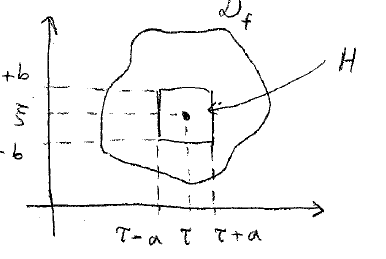
\includegraphics[width=.34\textwidth]{01_cauchy_peano_helyi_teglalap.png}
\end{center}
Mivel $f$ folytonos, a zárt téglalapon korlátos:
\[
 M:=\max_{H}\|f\|,\qquad
 \alpha:=\min\!\left\{a,\frac bM\right\}.
\]
Így igazolható, hogy a $[\tau-\alpha,\tau+\alpha]$
intervallumon van megoldás.

\noindent\textbf{2. megjegyzés:} a bizonyítás \textbf{nem konstruktív}.
Hivatkozás: Simon--Tóth, 40. oldal.

\subsubsection*{Vázlat: Arzelà--Ascoli-tétel}

Legyen $\Delta\subseteq\mathbb R$ korlátos, zárt intervallum,
$n\in\mathbb N$, és tekintsünk egy
\[
 (\varphi_k)_{k\in\mathbb N},\qquad
 \varphi_k:\Delta\to\mathbb R^n
\]
függvénysorozatot, amely
\begin{itemize}
 \item korlátos;
 \item egyenlő mértékben egyenletesen folytonos, azaz:
\end{itemize}
\[
 \begin{gathered}
 \forall\varepsilon>0\ \exists\delta>0\ \forall k\in\mathbb N\ 
 \forall t_1,t_2\in\Delta:\\[-1pt]
 |t_1-t_2|<\delta\quad\Longrightarrow\quad
 \|\varphi_k(t_1)-\varphi_k(t_2)\|_\infty<\varepsilon.
 \end{gathered}
\]
Ekkor a $(\varphi_k)$ sorozatnak $\exists$
\textbf{egyenletesen konvergens részsorozata}.

\subsubsection*{1. bizonyítás: Euler-féle törött vonalak}

A $[\tau,\tau+\alpha]$ intervallum egyenlő felosztása:
\[
 t_k=\tau+\alpha\frac{k}{N},\qquad k=1,2,\ldots,N-1.
\]
\begin{center}
 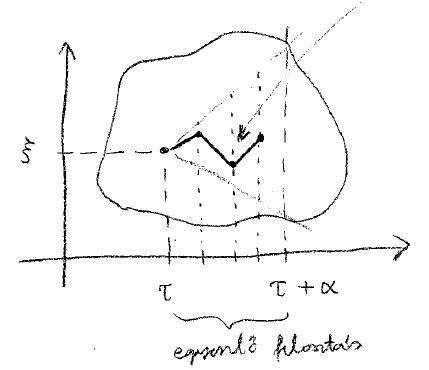
\includegraphics[width=.33\textwidth]{02_euler_torott_vonalak.png}
\end{center}
Az $(\varphi_N)$ Euler-féle töröttvonal-közelítések egyenlő
mértékben egyenletesen folytonosak. Ezért $\exists$ egy egyenletesen
konvergens részsorozat, amelynek határértéke megoldása
a kezdetiérték-problémának.

\subsubsection*{2. bizonyítás: Tonelli}

$N\in\mathbb N$ esetén a kéziratban szereplő közelítések:
\[
\boxed{\displaystyle
 x_N(t)=
 \begin{cases}
 \xi,
  & t\in\left[\tau,\tau+\frac{\alpha}{N}\right],\\[8pt]
 \displaystyle\xi+\int_\tau^{t-\frac\alpha N}
             f\bigl(s,x_{N-1}(s)\bigr)\,ds,
  & t\in\left[\tau+\frac\alpha N,\tau+\alpha\right].
 \end{cases}}
\]
Ekkor $x_N$ jól definiált. Az $(x_N)$ sorozat egyenlő
mértékben egyenletesen folytonos, ezért $\exists$ egyenletesen
konvergens részsorozata, amelynek határértéke a k.é.p. megoldása.

\subsection{A kezdetiérték-probléma megoldásának egyértelműsége}

\noindent\textbf{1. példa.} Az $x'=x$ egyenlet
\textbf{globálisan egyértelmű}, azaz minden leszűkítésre nézve
egyértelmű (lásd később).
\begin{center}
 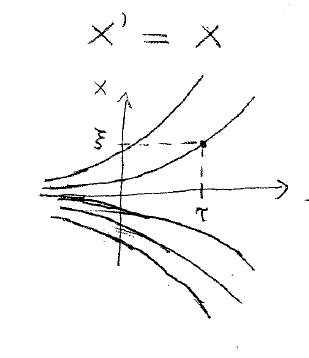
\includegraphics[width=.28\textwidth]{03_globalis_egyertelmuseg.png}
\end{center}

\noindent\textbf{2. példa.} Az $x'=\sqrt{|x|}$ egyenlet
\textbf{nem globálisan egyértelmű}, de a megjelölt pozitív
kezdeti értéknél \textbf{lokálisan egyértelmű}.
Ha $\xi=0$, akkor lokálisan sem egyértelmű.
\begin{center}
 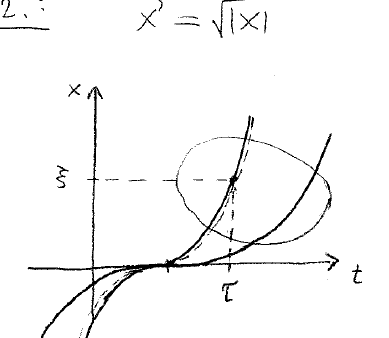
\includegraphics[width=.32\textwidth]{04_lokalis_egyertelmuseg.png}
\end{center}

\subsubsection*{Globális egyértelműség és teljes megoldás}

Az $x'=f\circ(\operatorname{id},x)$, $x(\tau)=\xi$
kezdetiérték-probléma \textbf{globálisan egyértelmű}, ha
bármely két $\varphi,\psi$ megoldásra
\[
  \varphi(t)=\psi(t)\qquad
  \forall\,\text{minden }t\in D_\varphi\cap D_\psi\text{ esetén}.
\]
Ezzel ekvivalens, hogy létezik egy nyílt
$\widetilde I\subseteq\mathbb R$ intervallum és egy
$\widetilde\varphi:\widetilde I\to\mathbb R^n$ megoldás úgy,
hogy $\forall$ minden más megoldás a $\widetilde\varphi$ valamely leszűkítése.
Ekkor $\widetilde\varphi$ a k.é.p. \textbf{teljes megoldása}.

\noindent\textbf{Megjegyzés.} A bizonyítás meggondolható.

\subsubsection*{Maximális megoldás}

A $\varphi^*:I^*\to\mathbb R^n$ függvény a k.é.p.
\textbf{maximális megoldása}, ha
\begin{enumerate}
 \item $\varphi^*$ megoldás $I^*$-on;
 \item nincs a k.é.p.-nak olyan, $\varphi^*$-tól különböző megoldása,
       amelynek leszűkítése a $\varphi^*$.
\end{enumerate}

\noindent\textbf{Megjegyzés.} Ha $\varphi$ teljes megoldás,
akkor maximális megoldás is (a fordított állítás nem szerepel a kéziratban).

\subsubsection*{Lokális egyértelműség}

A k.é.p. \textbf{lokálisan egyértelmű}, ha létezik
$K(\tau,\xi)\subseteq\mathbb R\times\mathbb R^n$ környezet
úgy, hogy a k.é.p.-nak erre való leszűkítése már
globálisan egyértelműen oldható meg.

\noindent\textbf{Megjegyzés.} A lokális egyértelműségre vannak
jól használható tételek.

\noindent\textbf{Tétel.} Ha $\forall$ minden $(\tau,\xi)\in D_f$
esetén a k.é.p. lokálisan egyértelműen oldható meg,
akkor $\forall$ minden kezdetiérték-probléma globálisan is
egyértelműen oldható meg ($\exists$ teljes megoldás).

\noindent\textbf{Bizonyítás:} indirekt.

\noindent\textbf{Érdekes példa.} Létezik folytonos
$f:\mathbb R^2\to\mathbb R$ úgy, hogy minden k.é.p.-nak
van megoldása, de egyetlen pontban sem lokálisan egyértelmű.
(A kézirat ezt konkrét konstrukció nélkül közli.)

\subsection{A lokális egyértelműség elegendő feltétele}

\noindent\textbf{Probléma:} mi biztosítja a lokális egyértelműséget?
A feltételekhez még hozzá lehet jutni.

\subsubsection*{Lipschitz-feltétel a második változóban}

Legyen $f:D\to\mathbb R^n$, ahol
$D\subseteq\mathbb R\times\mathbb R^n$ tartomány.
Az $f$ függvény a $(\tau,\xi)\in D_f$ pontban
\textbf{a második változójában lokálisan Lipschitz-feltételnek
tesz eleget}, ha létezik egy $K(\tau,\xi)\subseteq D_f$
környezet és egy $L(\tau,\xi)>0$ szám úgy, hogy
\[
 \boxed{\displaystyle
 \|f(t,u)-f(t,v)\|\le L\cdot\|u-v\|}
\]
$\forall$ minden $(t,u),(t,v)\in K(\tau,\xi)$ esetén.
(A norma tetszőleges norma $\mathbb R^n$-en.)

\noindent\textbf{1. megjegyzés:}
\begin{center}
 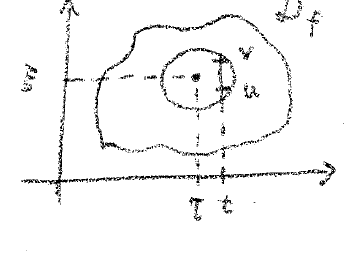
\includegraphics[width=.30\textwidth]{05_lipschitz_kornyezet.png}
\end{center}

\noindent\textbf{2. megjegyzés.} A Lipschitz-feltétel könnyen ellenőrizhető.

\noindent\textbf{Differenciálhatósági elegendő feltétel.}
Ha $D$ konvex és $f\in C^1(D)$, akkor $f$ $\forall$ minden
$D_f$-beli pontban lokálisan Lipschitz-feltételnek tesz eleget
második változójában.

\noindent\textbf{Emlékeztető: Lagrange-középértéktétel.}
Az $n=1$ esetben, ha $h\in C[a,b]$ és $h$ deriválható $(a,b)$-n,
akkor valamely $\eta\in(a,b)$ esetén
\[
 |h(b)-h(a)|=|h'(\eta)|\cdot|b-a|
 \le M\cdot|b-a|,
\]
ha $|h'|\le M$.
